\documentclass[a4paper,10pt]{article}
\usepackage[utf8x]{inputenc}
\usepackage{fullpage}
\usepackage{eurosym}
\usepackage{fullpage}
\usepackage{graphicx}
\usepackage{listings}
\lstset{
  language=Java,
  label=DescriptiveLabel,
  breaklines=true,
  showspaces=false,
  showstringspaces=false
}

%opening
\title{Open Information Systems Project - Conceptual Schema}
\author{Daniel Silva Chaltein de Almeida (98844)\\
Felipe Gomez Marulanda(92903)\\
Łukasz Kidziński (97612)\\
Thiago Mendonça (98255)\\
Wolney Mello Neto (98782)\\
\texttt{\{{}dsilvach,fegomezm,lkidzins,tdantasd,wdemello\}@vub.ac.be}}
\begin{document}

\maketitle

\section{Description}

We are proposing an ontology for RFPs\footnote{Request For Proposal} systems that manage movie rentals. Such systems would have the following process flow:
\begin{enumerate}
  \item Clients make requests: The client can either choose a specific movie or if he is uncertain about which movie to rent, choose some desired movie properties. The proposer will then recommend movies based on the constraints he defined.
    \subitem Constraints can be: genres, name of actors, director, year of release, etc.
    \subitem The client can also put a target price to pay (which can be accepted or raised by the proposer).
    \subitem Optionally, the client can also indicate until when he wishes to receive movie proposals, in case he wants the movies until a specific date.
  \item Video store owners look at the requests and make proposals, accepting the proposed price (if there is one) or adding their own price.
  \item Clients choose the best proposal
\end{enumerate}

Example:
\begin{enumerate}
  \item Client A makes a request for: 2 comedy movies with Jim Carrey and 1 Action movie from the previous year.
  \item Video store owners look at the request and make proposals: (Ace Ventura, The Mask and Inception for X \euro).
  \item Client A chooses one of the proposals and completes the transaction (or declines all the proposals).
\end{enumerate}

Ontology description:
\begin{itemize}
  \item At the time a request is made the client is not provided with the list of movies that match it. That list is part of the proposal and is going to be constructed by the video store owners. That is why every attribute of the Movie entity was attached to the Request entity.
  \item Only the most confusing entities have notes. Roles do not have them.
\end{itemize}

Figure \ref{fig:onto} shows the resulting ontology.

\begin{figure}[h!]
 \centering
  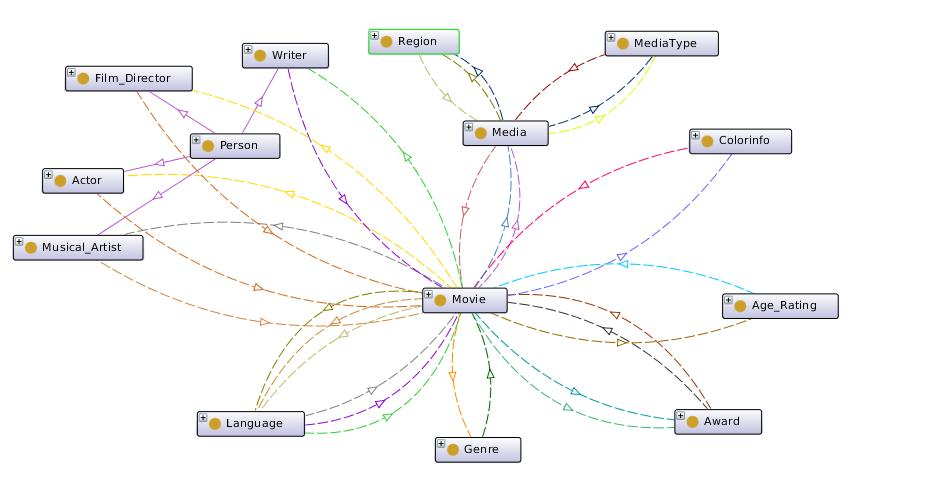
\includegraphics[width=\textwidth]{movie_ontology.jpg}
 \caption{Ontology constructed}
 \label{fig:onto}
\end{figure}



\section{Implementation}

This 3rd deliverable was implemented within two tools: Protégé\cite{protege} and Jena\cite{jena}. The former was used to build the ontology model in OWL\footnote{Web Ontology Language} while the latter was adopted to implement in Java the queries in SPARQL\footnote{SPARQL Protocol and RDF Query Language}.

\subsection{Building Ontology with Protégé}

We decided to build our ontology with the Protégé user interface. For this, we used the Movie Ontology as reference 
\cite{movieontology}. We implemented it using our vocabulary created with Collibra and reusing as many entities and 
properties as possible that appear on \cite{movieontology}, linking our data to theirs. The Movie Ontology, in turn, 
uses DBPedia \cite{dbpedia} for representing entities like \textbf{Language} and \textbf{Person}, moreover, it uses 
the W3C (Word Wide Web Consortium) \cite{w3c} for the \textbf{date} datatype. For identifying the \textbf{Movie} entity, we created an \textbf{imdb\_ID} property that has the ID of the Movie contained in the IMDb (Internet Movie Database).


\subsection{SPARQL Queries}
Some examples presented in Section 1 describe how an application would access the concepts defined in the movie ontology.
Therefore, SPARQL queries are implemented in order to make a demonstration of how these examples previously proposed work in practice.

Jena API was used to code a routine in Java composed by the following steps:

\begin{itemize}
  \item Load the model from an .owl file to create an instance of OntModel
\begin{lstlisting}
OntModel model = ModelFactory.createOntologyModel(OntModelSpec.OWL_DL_MEM_RDFS_INF);
// use the class loader to find the input file
InputStream in = FileManager.get().open(inputOWLFileName);
// read the RDF/XML/OWL file
model.read(new InputStreamReader(in), "");
\end{lstlisting}

  \item Write strings that are queries in SPARQL and submit them to QueryExecutionFactory
\begin{lstlisting}
String query2 = "SELECT ?p ?o WHERE {?p <http://www.movieontology.org/2009/10/01/movieontology.owl#
title> ?o.}";
\end{lstlisting}

  \item Collect the results from a ResultSet.
\begin{verbatim}
1 http://localhost/WTFDL/movie_ontology.owl#Way_of_the_Dragon Way of the Dragon 
2 http://localhost/WTFDL/movie_ontology.owl#The_Mask  The Mask  
3 http://localhost/WTFDL/movie_ontology.owl#Inception Inception 
4 http://localhost/WTFDL/movie_ontology.owl#Ace_Ventura Ace Ventura, Pet Detective  
\end{verbatim}

\end{itemize}

Furthermore, some other queries listed below were implemented:

\begin{itemize}

 \item Give me all the titles:
  \begin{itemize}
    \item Query : 
\begin{verbatim}
SELECT ?p ?o WHERE {?p <http://www.movieontology.org/2009/10/01/movieontology.owl#
title> ?o.}
\end{verbatim}
    \item Output
      \begin{verbatim}
1	http://localhost/WTFDL/movie_ontology.owl#Way_of_the_Dragon	Way of the Dragon	
2	http://localhost/WTFDL/movie_ontology.owl#The_Mask	The Mask	
3	http://localhost/WTFDL/movie_ontology.owl#Inception	Inception	
4	http://localhost/WTFDL/movie_ontology.owl#Ace_Ventura	Ace Ventura, Pet Detective	
      \end{verbatim}
    \end{itemize}

 \item Give me all titles containing ``the'':
  \begin{itemize}
    \item Query : 
\begin{verbatim}
SELECT ?p ?genre WHERE {
  ?p <http://www.movieontology.org/2009/10/01/movieontology.owl#
title> ?o.
FILTER regex(?o, "the", "i")
}
\end{verbatim}
    \item Output
      \begin{verbatim}
1 http://localhost/WTFDL/movie_ontology.owl#Way_of_the_Dragon 
2 http://localhost/WTFDL/movie_ontology.owl#The_Mask  
      \end{verbatim}
    \end{itemize}

 \item Give me 1 action movie from last year (2010):
  \begin{itemize}
    \item Query : 
\begin{verbatim}
PREFIX xsd: <http://www.w3.org/2001/XMLSchema#>
SELECT ?p ?date WHERE {?p <http://www.movieontology.org/2009/10/01/movieontology.owl#
belongsToGenre> <http://www.movieontology.org/2009/10/01/movieontology.owl#Action>.
?p <http://www.movieontology.org/2009/10/01/movieontology.owl#releasedate> ?date.
FILTER (?date >= "2010-01-01"^^xsd:date).}
LIMIT 1
\end{verbatim}
    \item Output
      \begin{verbatim}
1	http://localhost/WTFDL/movie_ontology.owl#Inception 2010-07-21^^
http://www.w3.org/2001/XMLSchema#date
      \end{verbatim}
    \end{itemize}

 \item Give me 2 comedy movies with Jim Carrey:
  \begin{itemize}
    \item Query : 
\begin{verbatim}
SELECT ?p WHERE {?p <http://www.movieontology.org/2009/10/01/movieontology.owl#
belongsToGenre> <http://www.movieontology.org/2009/10/01/movieontology.owl#Comedy>.
?p <http://www.movieontology.org/2009/10/01/movieontology.owl#hasActor>
<http://dbpedia.org/resource/Jim_Carrey>.}
LIMIT 2
\end{verbatim}
    \item Output
      \begin{verbatim}
1	http://localhost/WTFDL/movie_ontology.owl#The_Mask	
2	http://localhost/WTFDL/movie_ontology.owl#Ace_Ventura
      \end{verbatim}
    \end{itemize}

\end{itemize}

\appendix

\section{Ontology}

\lstinputlisting[language=XML]{../../ois/src/owl/movie_ontology.owl}

\bibliographystyle{plain}
\bibliography{biblio}

\end{document}
